\section{Inbetriebnahme}
Hier werden die Inbetriebnahmetests beschrieben.

\subsection{Tests Einzelkomponenten}

Kurz nach der Endmontage werden die einzelnen Komponenten getestet. Eine erste Inbetriebnahme des Ballnachschubs zeigt, das die Funktion gewährleistet ist. Das Drehmoment des Servomotors genügt um die 5 Bälle nach oben zu befördern. Die Geschwindigkeit des Ballnachschubs kann mit der Betriebsspannung des Motors eingestellt werden, allerdings ist sie auf ca. 12V begrenzt, da anderenfalls der Motor überlastet wird.

Der BLDC Motor kann bereits angesteuert werden und über ein Netzgerät wird die Drehzahl eingestellt. Hier zeigt sich, dass der Pneu eine Unwucht hat. Leider kann diese Unwucht nicht mit konventionellen Massnahmen behoben werden, das es sich um Ungenauigkeiten in der Dicke und in der Form handelt. Mit der erforderten Drehzahl für die Schussweite von ca. 2m wirkt sich die Unwucht jedoch nicht auf die Konstruktion aus.

Mit dieser Konfiguration werden die ersten Ballwürfe gemacht. Zuerst wird der Ballnachschub sehr langsam eingestellt, so dass die Drehzahl des Motors nach einem Schuss wieder auch die Anfangsdrehzahl gestiegen ist. Da die Streuung der Reichweite ungewöhnlich stark variiert (ca. 0.5m), haben wir auf der Gegenseite des Rades ein Stück Gummi aufgeklebt, so dass die Reibung des Tennisballs grösser ist. So wird die Streuung auf ca. 0.2m verkleinert. 

\begin{figure}[h!]          
	\centering             
	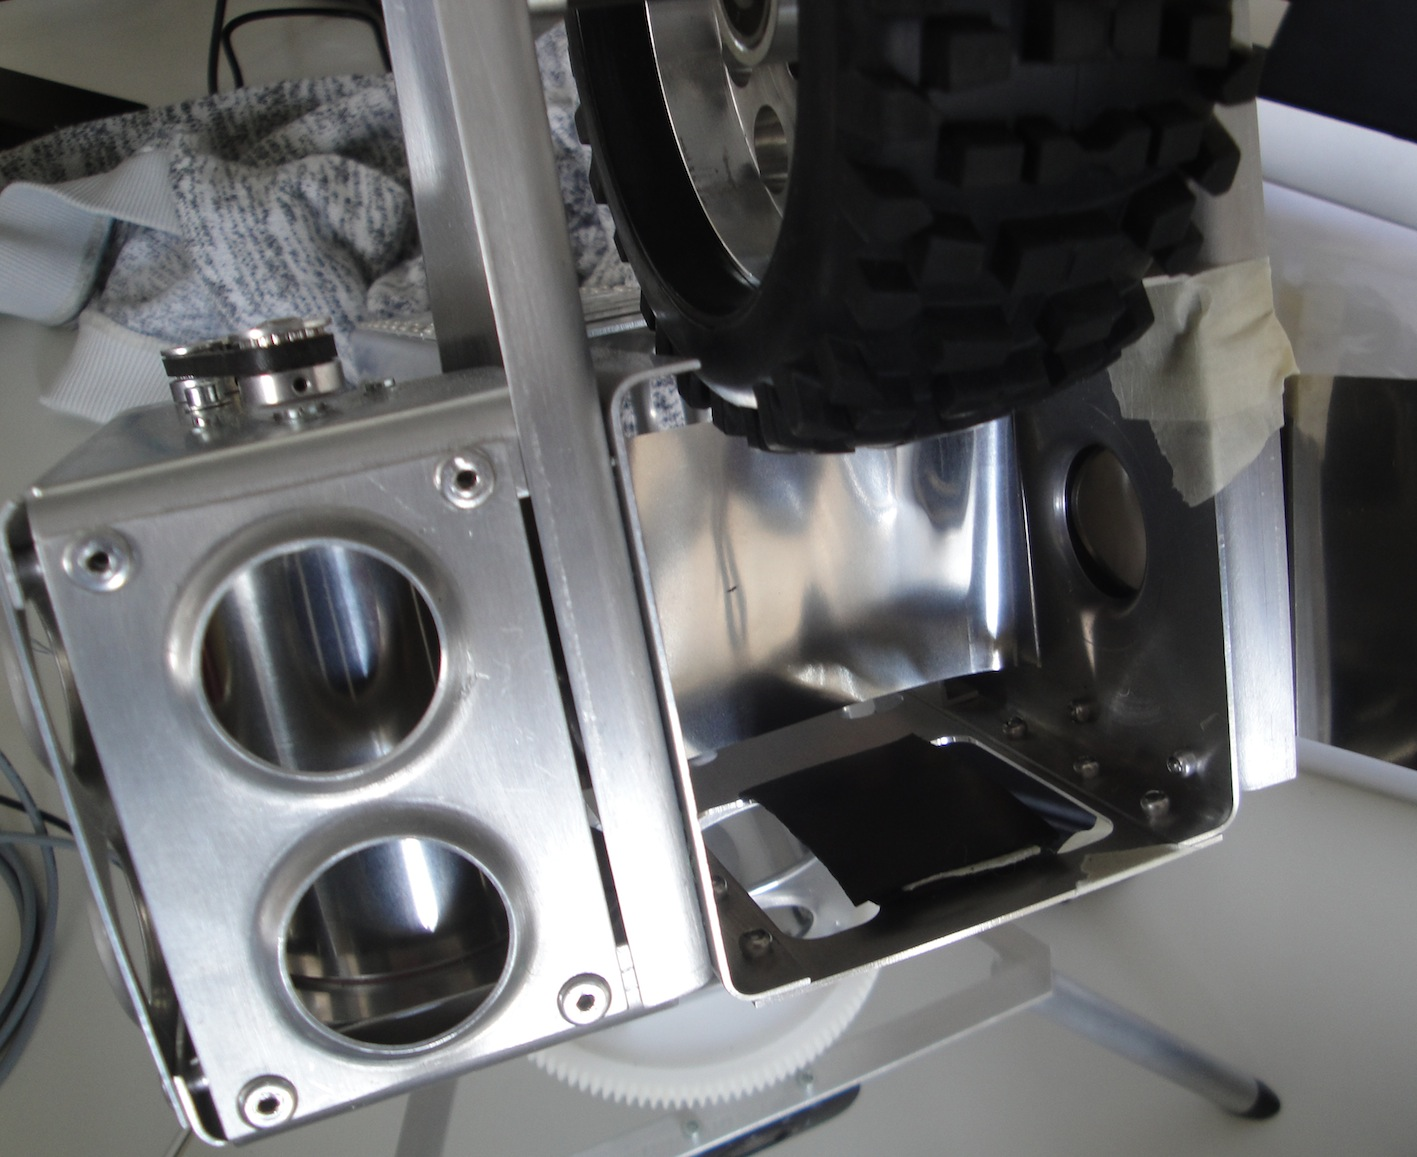
\includegraphics[width=0.5\textwidth]{fig/Bild_Gummi.JPG}
	\caption{Gummi zur Erhöhung der Reibung}
	\label{fig:Gummi}        
\end{figure}

In weiteren Tests werden die Bälle möglichst schnell nacheinander geschosssen, so dass sich die Drehzahl des BLDC Motors nicht mehr ganz erholen kann. Komischerweise wird so die Streuung noch kleiner (nicht mehr von Auge abschätzbar). Drei weitere Tests mit Wettbewerbsbedingungen (Distanz und Höhe des Korbes) und mit schnellem Ballnachschub zeigen, dass die Genauigkeit sehr hoch ist, alle Bälle landen im Korb. Gegebenenfalls könnte mit einem anderen Pneu die Genauigkeit noch erhöht werden.

Die Drehvorrichtung funktioniert, und ist sehr schnell. Bei ersten Tests (ohne Tennisbälle) konnte innerhalb einer Sekunde mehr als eine Umdrehung gemacht werden. Schlussendlich muss sich der Turm nur um ca. 16$^\circ$ drehen, somit sollten ca. 1/5 Sekunde reichen um die Richtung einzustellen.



\subsection{Tests System}

\subsection{Resultate}
